% Practice Test 07 — Minnesota Edition
% Questions: 30 (18 MC + 12 SA)
% Generated by scripts/generate_practice_tests.py

\begin{practiceQuestion}{1-3-q23}{sa}
\begin{questionText}
Two quantities are proportional with $k = 7$. If $y = 56$, what is $x$?
\end{questionText}
\correctAnswer{$x = 8$}
\explanation{$y = kx$ so $56 = 7x$, giving $x = 56 \div 7 = 8$.}
\end{practiceQuestion}

\begin{practiceQuestion}{1-5-q09}{mc}
\begin{questionText}
The point $(1, r)$ on a proportional graph represents:
\end{questionText}
\choiceA{The total amount}
\choiceB{The unit rate}
\choiceC{The number of units}
\choiceD{The $y$-intercept}
\correctAnswer{B}
\explanation{At $x = 1$, $y = k \times 1 = k$. So the $y$-value at $x = 1$ is the unit rate.}
\end{practiceQuestion}

\begin{practiceQuestion}{1-6-q29}{gsa}
\begin{questionText}
The double number line below relates inches on a blueprint to actual feet. A hallway measures $3.5$ inches on the blueprint. What is the actual length?

\begin{center}
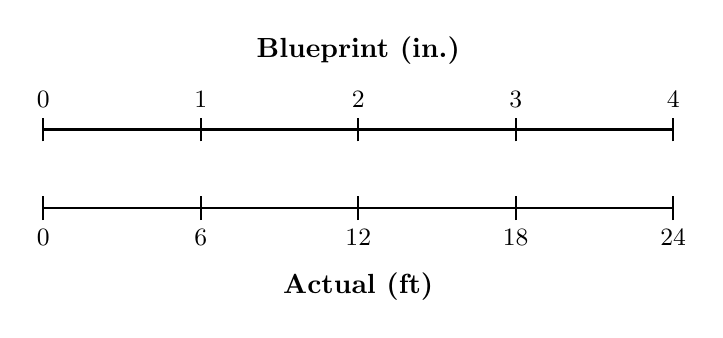
\begin{tikzpicture}[scale=1.0]
  % Top: blueprint inches
  \draw[thick] (0,1) -- (8,1);
  \foreach \x/\lab in {0/$0$, 2/$1$, 4/$2$, 6/$3$, 8/$4$} {
    \draw[thick] (\x,0.85) -- (\x,1.15);
    \node[above] at (\x,1.15) {\small \lab};
  }
  \node[above] at (4,1.7) {\textbf{Blueprint (in.)}};
  % Bottom: actual feet
  \draw[thick] (0,0) -- (8,0);
  \foreach \x/\lab in {0/$0$, 2/$6$, 4/$12$, 6/$18$, 8/$24$} {
    \draw[thick] (\x,-0.15) -- (\x,0.15);
    \node[below] at (\x,-0.15) {\small \lab};
  }
  \node[below] at (4,-0.7) {\textbf{Actual (ft)}};
\end{tikzpicture}
\end{center}
\end{questionText}
\correctAnswer{$21$ feet}
\explanation{Scale: $1$ inch $= 6$ feet. For $3.5$ inches: $6 \times 3.5 = 21$ feet.}
\end{practiceQuestion}

\begin{practiceQuestion}{2-1-q27}{gmc}
\begin{questionText}
The bar graph shows how many students chose each favorite sport. What percent of the students chose soccer?

\begin{center}
\begin{tikzpicture}[scale=0.55]
  \draw[thick,->] (0,0) -- (0,6.5) node[above]{\small Students};
  \draw[thick,->] (0,0) -- (7,0);
  % Bars
  \fill[funBlue!60] (0.5,0) rectangle (1.5,3);
  \fill[funGreen!60] (2,0) rectangle (3,6);
  \fill[funOrange!60] (3.5,0) rectangle (4.5,4.5);
  \fill[funRed!60] (5,0) rectangle (6,1.5);
  % Labels
  \node[below,font=\small] at (1,0) {Baseball};
  \node[below,font=\small] at (2.5,0) {Soccer};
  \node[below,font=\small] at (4,0) {Basketball};
  \node[below,font=\small] at (5.5,0) {Tennis};
  % Y-axis ticks
  \foreach \y/\lab in {1.5/6,3/12,4.5/18,6/24} {
    \draw (-0.1,\y) -- (0.1,\y) node[left,font=\small,xshift=-2pt] {\lab};
  }
  % Values on bars
  \node[above,font=\small] at (1,3) {$12$};
  \node[above,font=\small] at (2.5,6) {$24$};
  \node[above,font=\small] at (4,4.5) {$18$};
  \node[above,font=\small] at (5.5,1.5) {$6$};
\end{tikzpicture}
\end{center}
\end{questionText}
\choiceA{$24\%$}
\choiceB{$30\%$}
\choiceC{$40\%$}
\choiceD{$50\%$}
\correctAnswer{C}
\explanation{Total students: $12 + 24 + 18 + 6 = 60$. Soccer: $24$. Percent: $24 \div 60 = 0.40 = 40\%$.}
\end{practiceQuestion}

\begin{practiceQuestion}{2-5-q19}{sa}
\begin{questionText}
A dinner bill is $\$64$. You leave an $18\%$ tip. How much is the tip?
\end{questionText}
\correctAnswer{$\$11.52$}
\explanation{$64 \times 0.18 = \$11.52$.}
\end{practiceQuestion}

\begin{practiceQuestion}{2-7-q21}{sa}
\begin{questionText}
A baker expected to make $80$ cookies from a recipe but made $72$. What is the percent error (rounded to the nearest tenth)?
\end{questionText}
\correctAnswer{$\approx 11.1\%$}
\explanation{$\frac{|80 - 72|}{72} \times 100 = \frac{8}{72} \times 100 \approx 11.1\%$.}
\end{practiceQuestion}

\begin{practiceQuestion}{2-8-q12}{mc}
\begin{questionText}
You owe $\$250$ on a credit card with $20\%$ annual interest. If you pay nothing for $1$ year, how much will you owe?
\end{questionText}
\choiceA{$\$270$}
\choiceB{$\$300$}
\choiceC{$\$275$}
\choiceD{$\$350$}
\correctAnswer{B}
\explanation{Interest $= 250 \times 0.20 = \$50$. Total owed $= 250 + 50 = \$300$.}
\end{practiceQuestion}

\begin{practiceQuestion}{3-1-q04}{mc}
\begin{questionText}
A number plus its opposite always equals which value?
\end{questionText}
\choiceA{$1$}
\choiceB{$-1$}
\choiceC{The number itself}
\choiceD{$0$}
\correctAnswer{D}
\explanation{A number and its opposite are additive inverses. For example, $5 + (-5) = 0$.}
\end{practiceQuestion}

\begin{practiceQuestion}{4-1-q16}{mc}
\begin{questionText}
Evaluate $0.5n + 3.2$ when $n = 6$.
\end{questionText}
\choiceA{$6.2$}
\choiceB{$6.7$}
\choiceC{$9.2$}
\choiceD{$3.7$}
\correctAnswer{A}
\explanation{Substitute: $0.5(6) + 3.2 = 3.0 + 3.2 = 6.2$.}
\end{practiceQuestion}

\begin{practiceQuestion}{4-2-q08}{mc}
\begin{questionText}
Simplify $\frac{1}{3}x + \frac{2}{3}x$.


\begin{center}
\fractionCircle{1}{3}
\hspace{1cm}
\fractionCircle{2}{3}
\end{center}
\end{questionText}
\choiceA{$\frac{2}{9}x$}
\choiceB{$x$}
\choiceC{$\frac{3}{6}x$}
\choiceD{$\frac{1}{3}x^2$}
\correctAnswer{B}
\explanation{The coefficients are $\frac{1}{3}$ and $\frac{2}{3}$. Add: $\frac{1}{3} + \frac{2}{3} = \frac{3}{3} = 1$. Result: $1x = x$.}
\end{practiceQuestion}

\begin{practiceQuestion}{5-2-q13}{mc}
\begin{questionText}
You have $\$75$ in your bank account and withdraw $\$9$ each week. After how many weeks will you have $\$21$ left?
\end{questionText}
\choiceA{$5$ weeks}
\choiceB{$8$ weeks}
\choiceC{$7$ weeks}
\choiceD{$6$ weeks}
\correctAnswer{D}
\explanation{$75 - 9w = 21$. Subtract $75$: $-9w = -54$. Divide by $-9$: $w = 6$.}
\end{practiceQuestion}

\begin{practiceQuestion}{5-3-q17}{mc}
\begin{questionText}
Solve $-3(2n + 4) = -24$.
\end{questionText}
\choiceA{$n = 6$}
\choiceB{$n = -2$}
\choiceC{$n = 2$}
\choiceD{$n = 4$}
\correctAnswer{C}
\explanation{Divide by $-3$: $2n + 4 = 8$. Subtract $4$: $2n = 4$. Divide by $2$: $n = 2$. Check: $-3(2(2)+4) = -3(8) = -24$ \checkmark.}
\end{practiceQuestion}

\begin{practiceQuestion}{5-4-q20}{sa}
\begin{questionText}
Solve $0.75y + 2.25 = 8.25$.
\end{questionText}
\correctAnswer{$y = 8$}
\explanation{Subtract $2.25$: $0.75y = 6$. Divide by $0.75$: $y = 8$. Check: $0.75(8) + 2.25 = 6 + 2.25 = 8.25$ \checkmark.}
\end{practiceQuestion}

\begin{practiceQuestion}{5-5-q26}{gmc}
\begin{questionText}
Which inequality is represented by the number line below?

\begin{center}
\begin{tikzpicture}[scale=0.7]
  \draw[thick,->] (-1,0) -- (10,0);
  \foreach \x in {0,...,9} \draw (\x,0.15) -- (\x,-0.15) node[below] {$\x$};
  \draw[thick,funBlue,->] (5,0) -- (10,0);
  \draw[thick,funBlue,fill=white] (5,0) circle (4pt);
\end{tikzpicture}
\end{center}
\end{questionText}
\choiceA{$x \geq 5$}
\choiceB{$x > 5$}
\choiceC{$x \leq 5$}
\choiceD{$x < 5$}
\correctAnswer{B}
\explanation{An open circle at $5$ with shading to the right means $x > 5$ (not including $5$).}
\end{practiceQuestion}

\begin{practiceQuestion}{5-6-q29}{gsa}
\begin{questionText}
Solve $-3x + 9 > 0$. Then graph the solution on the number line below by describing the circle type and shading direction.

\begin{center}
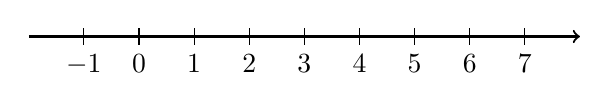
\begin{tikzpicture}[scale=0.7]
  \draw[thick,->] (-2,0) -- (8,0);
  \foreach \x in {-1,...,7} \draw (\x,0.15) -- (\x,-0.15) node[below] {$\x$};
\end{tikzpicture}
\end{center}
\end{questionText}
\correctAnswer{$x < 3$; open circle at $3$, shade left}
\explanation{Subtract $9$: $-3x > -9$. Divide by $-3$ and flip: $x < 3$. Open circle at $3$, shade left.}
\end{practiceQuestion}

\begin{practiceQuestion}{6-3-q30}{gsa}
\begin{questionText}
The diagram below shows a triangle attempt with the given side lengths. Explain whether this triangle is possible using the triangle inequality.

\begin{center}
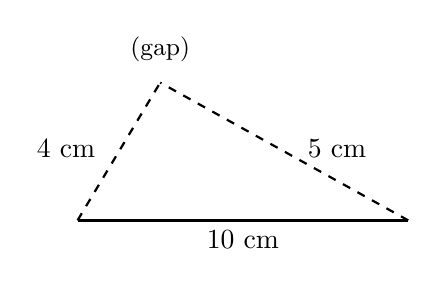
\begin{tikzpicture}[scale=0.7]
  \draw[thick] (0,0) -- (6,0);
  \draw[thick,dashed] (0,0) -- (1.5,2.5);
  \draw[thick,dashed] (6,0) -- (1.5,2.5);
  \node[below] at (3,0) {$10$ cm};
  \node[left] at (0.5,1.3) {$4$ cm};
  \node[right] at (4,1.3) {$5$ cm};
  \node[above] at (1.5,2.7) {\small (gap)};
\end{tikzpicture}
\end{center}
\end{questionText}
\correctAnswer{No, it is not possible}
\explanation{Check: $4 + 5 = 9 < 10$. The two shorter sides cannot connect across the base. The triangle inequality fails, so no triangle can be formed. The dashed lines with the gap illustrate that the sides don't meet.}
\end{practiceQuestion}

\begin{practiceQuestion}{6-4-q24}{sa}
\begin{questionText}
You are given two sides ($5$ cm and $7$ cm) and the included angle ($90°$). Is the resulting triangle unique? What type of triangle is it?
\end{questionText}
\correctAnswer{Yes, unique; it is a right triangle}
\explanation{SAS produces a unique triangle. The included angle of $90°$ makes it a right triangle with legs $5$ cm and $7$ cm.}
\end{practiceQuestion}

\begin{practiceQuestion}{6-5-q19}{sa}
\begin{questionText}
What shape is the cross-section when you cut a sphere through its center?
\end{questionText}
\correctAnswer{A circle (the largest possible circle)}
\explanation{A cut through the center of a sphere produces a great circle — the largest possible circular cross-section, with the same radius as the sphere.}
\end{practiceQuestion}

\begin{practiceQuestion}{6-6-q13}{mc}
\begin{questionText}
Two lines intersect. One angle formed is $130°$. What are the measures of all four angles?
\end{questionText}
\choiceA{$130°$, $130°$, $50°$, $50°$}
\choiceB{$130°$, $50°$, $130°$, $100°$}
\choiceC{$130°$, $130°$, $130°$, $130°$}
\choiceD{$130°$, $60°$, $130°$, $40°$}
\correctAnswer{A}
\explanation{Vertical angles are equal ($130°$ and $130°$). Adjacent angles are supplementary: $180° - 130° = 50°$. The four angles are $130°$, $50°$, $130°$, $50°$.}
\end{practiceQuestion}

\begin{practiceQuestion}{7-3-q16}{mc}
\begin{questionText}
A student says the area of a circle with radius $6$ cm is $37.68$ cm$^2$. What mistake did the student most likely make?
\end{questionText}
\choiceA{Used diameter instead of radius}
\choiceB{Calculated circumference instead of area}
\choiceC{Forgot to square the radius}
\choiceD{Divided by $2$ instead of squaring}
\correctAnswer{B}
\explanation{$C = 2\pi r = 2 \times 3.14 \times 6 = 37.68$. The student found circumference, not area. The area is $3.14 \times 36 = 113.04$ cm$^2$.}
\end{practiceQuestion}

\begin{practiceQuestion}{7-4-q09}{mc}
\begin{questionText}
A banner is shaped like a rectangle $18$ in by $6$ in with a triangle cut from one end. The triangle has a base of $6$ in and a height of $4$ in. What is the area of the banner?
\end{questionText}
\choiceA{$84$ in$^2$}
\choiceB{$96$ in$^2$}
\choiceC{$108$ in$^2$}
\choiceD{$120$ in$^2$}
\correctAnswer{B}
\explanation{Rectangle: $18 \times 6 = 108$ in$^2$. Triangle: $\frac{1}{2} \times 6 \times 4 = 12$ in$^2$. Banner: $108 - 12 = 96$ in$^2$.}
\end{practiceQuestion}

\begin{practiceQuestion}{7-5-q12}{mc}
\begin{questionText}
A storage box is in the shape of a cube with side $12$ inches. What is its surface area?
\end{questionText}
\choiceA{$144$ in$^2$}
\choiceB{$432$ in$^2$}
\choiceC{$864$ in$^2$}
\choiceD{$1728$ in$^2$}
\correctAnswer{C}
\explanation{$SA = 6s^2 = 6 \times 144 = 864$ in$^2$.}
\end{practiceQuestion}

\begin{practiceQuestion}{7-6-q08}{mc}
\begin{questionText}
A storage container is $2$ ft long, $1.5$ ft wide, and $3$ ft tall. How many cubic feet can it hold?
\end{questionText}
\choiceA{$6$ ft$^3$}
\choiceB{$6.5$ ft$^3$}
\choiceC{$9$ ft$^3$}
\choiceD{$10$ ft$^3$}
\correctAnswer{C}
\explanation{$V = 2 \times 1.5 \times 3 = 9$ ft$^3$.}
\end{practiceQuestion}

\begin{practiceQuestion}{8-1-q26}{gmc}
\begin{questionText}
A student surveyed $50$ classmates about their favorite fruit. The results are shown in the bar graph below.

\begin{center}
\begin{tikzpicture}[scale=0.7]
  \draw[thick,->] (0,0) -- (0,6.5) node[above]{\small Number of Students};
  \draw[thick,->] (0,0) -- (8.5,0);
  % bars
  \fill[funBlue!70] (0.5,0) rectangle (1.5,4);
  \fill[funGreen!70] (2.5,0) rectangle (3.5,3);
  \fill[funOrange!70] (4.5,0) rectangle (5.5,2);
  \fill[funRed!70] (6.5,0) rectangle (7.5,1);
  % labels
  \node[below] at (1,0) {\small Apple};
  \node[below] at (3,0) {\small Banana};
  \node[below] at (5,0) {\small Orange};
  \node[below] at (7,0) {\small Grape};
  % y-axis ticks
  \foreach \y in {1,2,3,4,5,6} {
    \draw (-0.1,\y) -- (0.1,\y);
    \node[left] at (0,\y) {\small $\y\times5$};
  }
  % values on bars
  \node[above] at (1,4) {\small $20$};
  \node[above] at (3,3) {\small $15$};
  \node[above] at (5,2) {\small $10$};
  \node[above] at (7,1) {\small $5$};
\end{tikzpicture}
\end{center}

If there are $500$ students in the school, predict how many prefer apples.
\end{questionText}
\choiceA{$20$}
\choiceB{$100$}
\choiceC{$200$}
\choiceD{$250$}
\correctAnswer{C}
\explanation{$\frac{20}{50} = 40\%$ prefer apples. $40\%$ of $500 = 200$.}
\end{practiceQuestion}

\begin{practiceQuestion}{8-3-q13}{mc}
\begin{questionText}
The difference between the means of two groups is $10$. The MAD for each group is $2$. How many MADs apart are the means?
\end{questionText}
\choiceA{$2$}
\choiceB{$5$}
\choiceC{$10$}
\choiceD{$20$}
\correctAnswer{B}
\explanation{$\frac{10}{2} = 5$ MADs apart.}
\end{practiceQuestion}

\begin{practiceQuestion}{8-4-q15}{mc}
\begin{questionText}
Why is it important to use multiple measures (mean, median, range, IQR, MAD) when comparing two groups?
\end{questionText}
\choiceA{One measure tells the complete story}
\choiceB{Using more measures wastes time}
\choiceC{Different measures reveal different aspects of the data}
\choiceD{All measures always give the same conclusion}
\correctAnswer{C}
\explanation{Mean and median show center; range, IQR, and MAD show spread. Together they give a complete picture.}
\end{practiceQuestion}

\begin{practiceQuestion}{8-6-q19}{sa}
\begin{questionText}
A circle graph shows $35\%$ for music, $25\%$ for art, and the rest for drama. What percent is drama?
\end{questionText}
\correctAnswer{$40\%$}
\explanation{$100\% - 35\% - 25\% = 40\%$.}
\end{practiceQuestion}

\begin{practiceQuestion}{9-4-q30}{gsa}
\begin{questionText}
The table below shows a probability model for a game spinner. One probability is missing. Find the missing probability for outcome D.

\begin{center}
\begin{tabular}{|c|c|}
\hline
\textbf{Outcome} & \textbf{Probability} \\
\hline
A & $0.30$ \\
\hline
B & $0.25$ \\
\hline
C & $0.15$ \\
\hline
D & ? \\
\hline
\end{tabular}
\end{center}
\end{questionText}
\correctAnswer{$0.30$}
\explanation{$P(D) = 1 - (0.30 + 0.25 + 0.15) = 1 - 0.70 = 0.30$.}
\end{practiceQuestion}

\begin{practiceQuestion}{9-6-q06}{mc}
\begin{questionText}
Two dice are rolled. What is the probability that both dice show the same number (doubles)?
\end{questionText}
\choiceA{$\frac{1}{36}$}
\choiceB{$\frac{1}{12}$}
\choiceC{$\frac{1}{6}$}
\choiceD{$\frac{1}{3}$}
\correctAnswer{C}
\explanation{Doubles: $(1,1), (2,2), (3,3), (4,4), (5,5), (6,6)$ — that is $6$ out of $36$. $P = \frac{6}{36} = \frac{1}{6}$.}
\end{practiceQuestion}

\begin{practiceQuestion}{9-7-q25}{sa}
\begin{questionText}
A student runs $200$ simulation trials for an event with theoretical probability $\frac{1}{4}$. They observe the event $54$ times. What is the experimental probability? Is it close to the theoretical value?
\end{questionText}
\correctAnswer{$0.27$; yes, it is close to $0.25$}
\explanation{$P = \frac{54}{200} = 0.27$. Theoretical $= 0.25$. The difference of $0.02$ is small, especially with $200$ trials.}
\end{practiceQuestion}
